\documentclass[crop,class=article]{standalone}
%----------------------------Preamble-------------------------------%
\usepackage{tikz}                       % Drawing/graphing tools.
\usetikzlibrary{
    arrows.meta,            % Latex and Stealth arrows.
    decorations.markings    % Adding arrows in the middle of a line.
}
%--------------------------Main Document----------------------------%
\begin{document}
    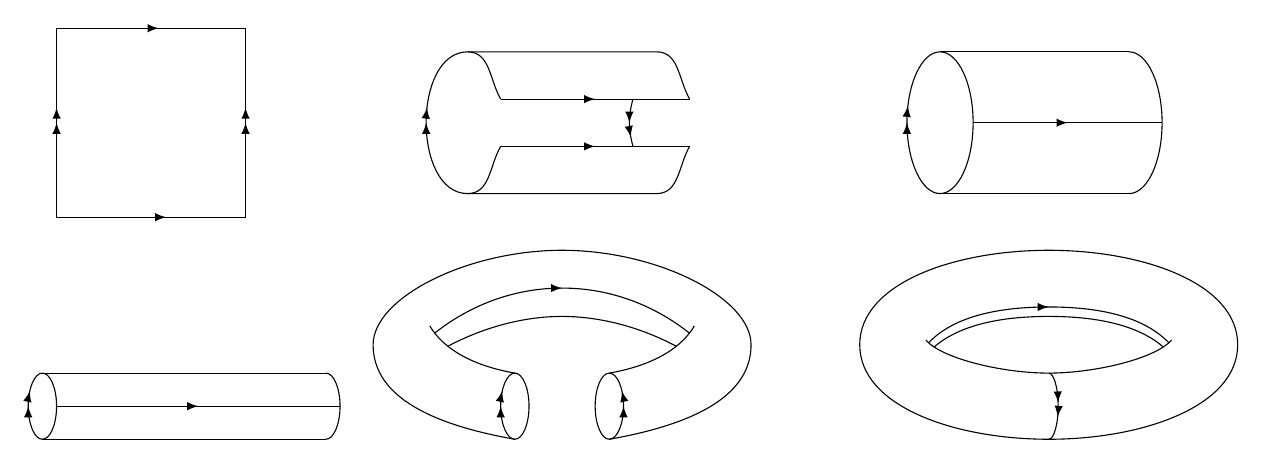
\begin{tikzpicture}[scale=1.2]
        % Draw square.
        \draw[%
            postaction={decorate},
            decoration={%
                markings,
                mark=at position .145 with \arrow{latex},
                mark=at position .375 with \arrow{latex},
                mark=at position .395 with \arrow{latex},
                mark=at position .615 with \arrowreversed{latex},
                mark=at position .855 with \arrowreversed{latex},
                mark=at position .875 with \arrowreversed{latex}
            }
        ]   (0,-1) -- (2,-1) -- (2,1) -- (0,1) -- cycle;

        % Draw squaring folding into cylinder.
        \begin{scope}[xshift=4.7cm]
            \draw[%
                postaction={decorate},
                decoration={%
                    markings,
                    mark=at position .5 with \arrow{latex}
                }
            ]   (0,0.25) -- (2,0.25);
            \draw[%
                postaction={decorate},
                decoration={%
                    markings,
                    mark=at position .5 with \arrow{latex}
                }
            ]   (0,-.25) -- (2,-0.25);
            \draw[%
                postaction={decorate},
                decoration={%
                    markings,
                    mark=at position .5 with \arrow{latex},
                    mark=at position .55 with \arrow{latex}
                }
            ]
                (0,-.25) to [out=-120,in=0] (-.35,-.75)
                         to [out=180,in=180] (-.35,.75)
                         to [out=0,in=120] (0,.25);
            \draw (2,.25) to [out=120,in=0] (1.65,0.75)
                          to (-0.35,0.75);
            \draw (-0.35,-0.75) to (1.65,-0.75)
                                to [out=0,in=-120] (2,-0.25);
            \draw[%
                postaction={decorate},
                decoration={%
                    markings,
                    mark=at position .5 with \arrow{latex},
                    mark=at position .8 with \arrow{latex}
                }
            ]
                (1.4,0.25) to [out=-105,in=105] (1.4,-0.25);
        \end{scope}

        % Draw cylinder.
        \begin{scope}[xshift=9.7cm]
            \draw[%
                postaction={decorate},
                decoration={%
                    markings,
                    mark=at position .5 with \arrow{latex}
                }
            ]   (0,0) -- (2,0);
            \draw[%
                postaction={decorate},
                decoration={%
                    markings,
                    mark=at position .5 with \arrow{latex},
                    mark=at position .55 with \arrow{latex}
                }
            ]   (0,0)
                arc[%
                    start angle=0,
                    delta angle=-360,
                    x radius=.35,
                    y radius=.75
                ];
            \draw   (1.65,-0.75) arc[%
                        start angle=-90,
                        delta angle=180,
                        x radius=.35,
                        y radius=.75
                    ];
            \draw (-0.35,-0.75) -- (1.65,-0.75);
            \draw (-0.35,0.75) -- (1.65,0.75);
        \end{scope}

        % Draw stretched out cylinder.
        \begin{scope}[yshift=-3cm]
            \draw[%
                postaction={decorate},
                decoration={%
                    markings,
                    mark=at position .5 with \arrow{latex}
                }
            ]   (0,0) -- (3,0);
            \draw[%
                postaction={decorate},
                decoration={%
                    markings,
                    mark=at position .5 with \arrow{latex},
                    mark=at position .6 with \arrow{latex}
                }
            ]   (0,0) arc[%
                    start angle=0,
                    delta angle=-360,
                    x radius=.15,
                    y radius=.35
                ];
            \draw (2.85,0.35) arc[%
                        start angle=90,
                        delta angle=-180,
                        x radius=.15,
                        y radius=.35
                    ];
            \draw (-0.15,0.35) -- (2.85,0.35);
            \draw (-0.15,-0.35) -- (2.85,-0.35);
        \end{scope}

        % Draw cylinder bending into torus.
        \begin{scope}[xshift=4cm, yshift=-3cm]
            \draw[%
                postaction={decorate},
                decoration={%
                    markings,
                    mark=at position .5 with \arrow{latex},
                    mark=at position .6 with \arrow{latex}
                }
            ]   (1,0 ) arc[%
                    start angle=0,
                    delta angle=-360,
                    x radius=.15,
                    y radius=.35
                ];
            \draw (0.85,-0.35)..controls +(170:1) and +(-90:.5) 
                ..(-0.65,0.65)..controls +(90:.5) and +(180:1)
                ..(1.35,1.65)..controls +(0:1) and +(90:.5)
                ..(3.35,0.65)..controls +(-90:.5) and +(10:1)
                ..(1.85,-0.35);
            \draw[%
                postaction={decorate},
                decoration={%
                    markings,
                    mark=at position .5 with \arrow{latex},
                    mark=at position .6 with \arrow{latex}
                }
            ]   (1.7,0.0) arc[%
                    start angle=0,
                    delta angle=-360,
                    x radius=-.15,
                    y radius=.35
                ];
            \draw (0.85,0.35)..controls +(170:.5) and +(-60:.25)
                ..(-.05,.85);
            \draw (1.85,0.35)..controls +(10:.5) and +(240:.25)
                ..(2.75,.85);
            \clip (0.85,0.35)..controls +(170:.5) and +(-60:.25)
                ..(-0.05,0.85) -- (-0.05,1.4) -|
                  (2.75,0.85)..controls +(240:.25) and +(10:.5)
                ..(1.85,0.35);
            \draw (-0.65,-0.25)..controls +(90:.5) and +(180:1)
                ..(1.35,0.95)..controls +(0:1) and +(90:.5)
                ..(3.35,-0.25);
            \draw[%
                postaction={decorate},
                decoration={%
                    markings,
                    mark=at position .5 with \arrow{latex}
                }
            ]   (-0.65,-.25)..controls +(90:.5) and +(180:1.2)..
                (1.35,1.25)..controls +(0:1.2) and +(90:.5)..
                (3.35,-0.25);
        \end{scope}

        % Draw torus.
        \begin{scope}[xshift=9cm, yshift=-3cm]
            \draw[%
                postaction={decorate},
                decoration={%
                    markings,
                    mark=at position .45 with \arrow{latex},
                    mark=at position .65 with \arrow{latex}
                }
            ]   (1.5,.35) arc[%
                    start angle=90,
                    end angle=-90,
                    y radius=.35,
                    x radius=.1
                ];
            \draw (1.5,-.35)..controls +(180:1) and +(-90:.65)
                ..(-0.5,0.65)..controls +(90:.65) and +(180:1)
                ..(1.5,1.65)..controls +(0:1) and +(90:.65)
                ..(3.5,0.65)..controls +(-90:.65) and +(0:1)
                ..cycle;
            \draw (1.5,.35)..controls +(180:.5) and +(-50:.25)
                ..(0.2,0.7);
            \draw (1.5,.35)..controls +(0:.5) and +(230:.25)
                ..(2.8,.7);
            \clip (1.5,.35)..controls +(180:.5) and +(-50:.25)
                ..(0.2,0.7) -- (0.2,1.2) -|
                  (2.8,.7)..controls +(230:.25) and +(0:.5)
                ..(1.5,0.35);
            \draw (0,-0.05)..controls +(90:.65) and +(180:1)
                ..(1.5,0.95)..controls +(0:1) and +(90:.65)
                ..(3,-0.05);
            \draw[%
                postaction={decorate},
                decoration={%
                    markings,
                    mark=at position .5 with \arrow{latex}
                    }
            ]   (0,0.05)..controls +(90:.65) and +(180:1)
              ..(1.5,1.05)..controls +(0:1) and +(90:.65)
              ..(3,0.05);
        \end{scope}
    \end{tikzpicture}
\end{document}